%
% NOTE -- ONLY EDIT THE .Rnw FILE!!!  The .tex file is
% likely to be overwritten.
%
%\VignetteIndexEntry{GLIDE}
%\VignetteDepends{}
%\VignetteKeywords{Documentation}
%\VignettePackage{GLIDE}
\documentclass[12pt]{article}
\usepackage{times}
\usepackage{hyperref}
%\usepackage[authoryear,round]{natbib}

\textwidth=6.2in
\textheight=8.5in
%\parskip=.3cm
\oddsidemargin=.1in
\evensidemargin=.1in
\headheight=-.3in

\newcommand{\scscst}{\scriptscriptstyle}
\newcommand{\scst}{\scriptstyle}

\newcommand{\R}{{\textsf{R}}}
\newcommand{\code}[1]{{\texttt{#1}}}
\newcommand{\term}[1]{{\emph{#1}}}
\newcommand{\Rpackage}[1]{\textsf{#1}}
\newcommand{\Rfunction}[1]{\texttt{#1}}
\newcommand{\Robject}[1]{\texttt{#1}}
\newcommand{\Rclass}[1]{{\textit{#1}}}
\newcommand{\Rmethod}[1]{{\textit{#1}}}
\newcommand{\Rfunarg}[1]{{\textit{#1}}}

%\bibliographystyle{plainnat}

\usepackage{Sweave}
\begin{document}
\Sconcordance{concordance:GLIDE.tex:GLIDE.Rnw:%
1 35 1 1 0 29 1 1 5 4 1 1 2 1 0 3 1 9 0 1 3 1 1 1 2 4 0 1 2 1 1 1 2 1 0 %
1 1 6 0 1 2 1 1 1 3 19 0 1 1 19 0 1 2 4 1 1 9 7 1 1 2 19 0 1 2 6 1}















\title{The \Rpackage{GLIDE} package: Global and Individual Tests for Direct Effects}
\author{Xiaoyu Wang, James Y. Dai}
\maketitle

\section{Introduction}

``Mendelian randomization'', an inferential method that uses germline genotypes as instrumental variables (IVs) to study the environmentally modifiable cause of human disease, has been increasingly popular in genetic epidemiology. Exploiting the random assortment of genes from parents to offsprings at the time of gamete formation, likened to ``Nature$\prime$s randomized experiment'', Mendelian randomization holds promise for removing confounding and reverse causation that loom over observational epidemiology. While conceptually appealing, skepticism has persisted on feasibility of strong assumptions required by Mendelian randomization, stated informally, that genetic variants are independent of confounders of the exposuredisease relation, that genetic variants are associated with the exposure, preferably strongly, and that there is no direct effect from genetic variants to the disease other than the pathway through the exposure, also known as no ``pleiotropy''. As the founding principle, the independence assumption is largely backed by random meiosis and further aided by adjustment for population substructures. The strength of IVs can be somewhat improved by inclusion of tens and hundreds of known risk loci identified by genome-wide association studies with increasingly larger sample sizes. Perhaps the Achilles$\prime$ heel for Mendelian randomization is potential pleiotropic effects among candidate genetic IVs, which can be sometimes plausible given complex biological pathways and networks. This threat to the validity of Mendelian randomization is heightened by the very practice of including a large number of risk variants to boost the strength of IVs.

Take current investigations on body mass index (BMI) and risk of colorectal cancer for example. Using seventy seven genome-wide significant SNPs for high BMI in the GIANT consortium study, several Mendelian randomization studies have reported strong evidence of causal relationship between BMI and colorectal cancer risk. However, as revealed by the GIANT consortium study, BMI is one of many metabolic phenotypes, and many BMI-associated SNPs are also associated with other metabolic phenotypes such as type2 diabetes, higher high-density lipoprotein cholesterol (HDL), and coronary artery diseases (CAD). Pathway analysis therein suggested that risk loci involve in central nervous system, glutamate signalling, energy metabolism, lipid biology and adipogenesis, underscoring the heterogeneous aetiology of obesity. Possibility of pleiotropy for these 77 SNPs, or a subset of them, is not dismissable. Methodologies for detecting pleiotropy and, more ambitiously, estimating causal effect in the presence of pleiotropy have been under active development. 

we propose \Rpackage{GLIDE}, GLobal and Individual tests for Direct Effects, a statistical method to assess pleiotropy and refine IVs for Mendelian randomization. Causal effects are defined in relative risk, a measure that is collapsible and well interpretable for binary disease endpoints. Though not all direct effects defined in a joint causal model are identifiable, we show that ``marginal'' direct effects, the direct effect for one individual variant that is not conditional on other direct effects, are estimable and provide valid tests for individual direct effects. A quantile-quantile plot is proposed to examine the degree of pleiotropy graphically. A parametric simulation procedure gives the significance of pleiotropic effect for any given variant, as well as evidence of global violation. Based on the proposed method, investigators can determine whether the set of genetic variants being considered for IVs are grossly invalid, or a subset of them appears trustworthy for Mendelian randomization. Our comprehensive simulation results suggest that the proposed test is nearly uniformly more sensitive than the Egger regression. When used to reanalyze BMI, height and colorectal cancer risk in the Genetics and Epidemiology of Colorectal Cancer Consortium (GECCO), our method suggests that at least several variants among the SNPs being used as IVs exhibit strong evidence of pleiotropy and therefore should be excluded in Mendelian randomization.




\section{Main function}

We show an example of applying the function on a dataset from GECCO. 
First we load the example dataset:
\begin{Schunk}
\begin{Sinput}
> data(BMI)
> str(exposure_coeff)
\end{Sinput}
\begin{Soutput}
 Named num [1:77] 0.0192 0.023 0.0229 0.0307 0.0174 0.0402 0.0249 0.0414 0.0307 0.0207 ...
 - attr(*, "names")= chr [1:77] "rs1000940" "rs10132280" "rs1016287" "rs10182181" ...
\end{Soutput}
\begin{Sinput}
> dim(dat)
\end{Sinput}
\begin{Soutput}
[1] 20515    84
\end{Soutput}
\end{Schunk}

We find the columns in dat that contain genotype data:
\begin{Schunk}
\begin{Sinput}
> genotype_columns=which(grepl("^rs",colnames(dat)))
\end{Sinput}
\end{Schunk}

We feed in the formula of outcome ~ adjusting covariates:
\begin{Schunk}
\begin{Sinput}
> formula=as.formula("outcome~as.factor(gecco_study)+age_ref+sex+pc1+pc2+pc3")
> formula
\end{Sinput}
\begin{Soutput}
outcome ~ as.factor(gecco_study) + age_ref + sex + pc1 + pc2 + 
    pc3
\end{Soutput}
\end{Schunk}

We then run the glide function:
\begin{Schunk}
\begin{Sinput}
> out=glide(formula=formula,exposure_coeff=exposure_coeff,genotype_columns,data=dat,np=100000,qcutoff=0.2,parallel=TRUE,corenumber=4,verbose=TRUE)
\end{Sinput}
\begin{Soutput}
GLIDE program starts at: 2017-03-17 18:23:16
Warning message: 3 rows were removed due to missing data in age_ref
Compute the correlation matrix at: 2017-03-17 18:23:40
Total 77 iterations... 
There are 56 cores available in the machine.
Start parallel computation of the correlation matrix using 28 cores...
10 ..20 ..30 ..40 ..50 ..60 ..70 ..

Compute the null p-value at: 2017-03-17 18:24:04

Compute the FWER and FDR values at: 2017-03-17 18:24:20

GLIDE program ends at: 2017-03-17 18:24:32
\end{Soutput}
\begin{Sinput}
> head(out)
\end{Sinput}
\begin{Soutput}
           observed_pvalue expected_pvalue    fwer   q_value geffect_exposure
rs1000940        0.8906115       0.8591219 1.00000 0.9804136           0.0192
rs10132280       0.7896098       0.7567105 1.00000 0.9804136           0.0230
rs1016287        0.5432898       0.4746128 1.00000 0.9804136           0.0229
rs10182181       0.7719084       0.7182215 1.00000 0.9804136           0.0307
rs10733682       0.9295840       0.9360076 1.00000 0.9804136           0.0174
rs10938397       0.1196764       0.1284999 0.99994 0.8965644           0.0402
           geffect_outcome geffect_outcome_variance
rs1000940      0.008223924             0.0005346975
rs10132280     0.001237929             0.0004747197
rs1016287      0.019562750             0.0005130450
rs10182181     0.002487054             0.0004119974
rs10733682     0.003528327             0.0004280288
rs10938397     0.042404116             0.0004115602
\end{Soutput}
\end{Schunk}

\section{plot result}
We draw the q-q plot: plot.glide(out)
We draw the Egger plot: plot.egger(out)
The figures are shown as follows:
\begin{figure}[h]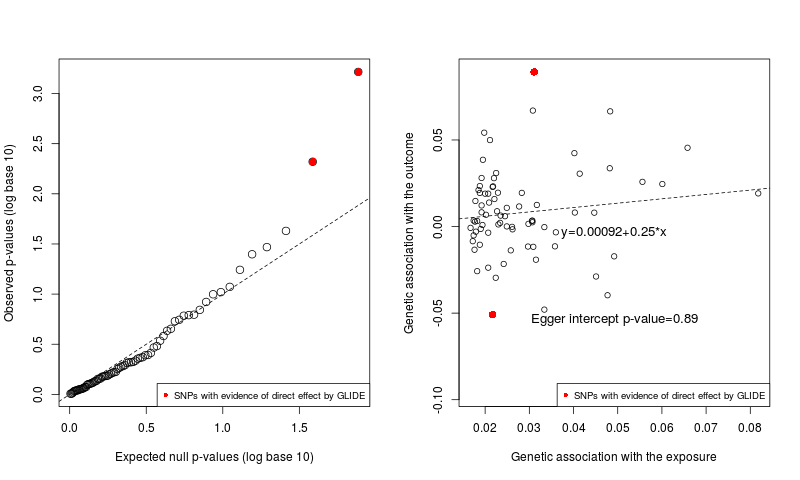
\includegraphics{./plot.png}\end{figure}
\section{session information}

The version number of \R{} and packages loaded for generating the vignette were:

\begin{verbatim}
R version 3.2.2 (2015-08-14)
Platform: x86_64-pc-linux-gnu (64-bit)
Running under: Ubuntu 14.04.3 LTS

locale:
 [1] LC_CTYPE=en_US.UTF-8       LC_NUMERIC=C              
 [3] LC_TIME=en_US.UTF-8        LC_COLLATE=en_US.UTF-8    
 [5] LC_MONETARY=en_US.UTF-8    LC_MESSAGES=en_US.UTF-8   
 [7] LC_PAPER=en_US.UTF-8       LC_NAME=C                 
 [9] LC_ADDRESS=C               LC_TELEPHONE=C            
[11] LC_MEASUREMENT=en_US.UTF-8 LC_IDENTIFICATION=C       

attached base packages:
[1] stats     graphics  grDevices utils     datasets  methods   base     

other attached packages:
[1] GLIDE_1.0.1

loaded via a namespace (and not attached):
[1] compiler_3.2.2   MASS_7.3-44      parallel_3.2.2   tools_3.2.2     
[5] codetools_0.2-14 iterators_1.0.7  foreach_1.4.2    doMC_1.3.3      \end{verbatim}

% \bibliographystyle{plain}
% \bibliography{GLIDE}

\end{document}
